% !TEX root = ../main.tex
\chapter{Twitter}
\label{ch:twitter}

\section{Introduction to Twitter}
\label{sec:twitter}

Twitter is a form of so-called microblogging, which is defined as a form of blogging with small-sized pieces of content,
usually text up to a character-count of 200, which in the case of Twitter are called Tweets or statuses.
This enables light-weight, mobile and easy sharing of opinions, status and activities~\cite{Finin2007},
which lead to rapid adoption and user growth~\cite{mcgiboney2009twitter}.
\par
As shown in~\ref{tab:comparison}, the relationships of following users and being followed by users on Twitter is unreciprocated,
which means it requires no active accepting of followers.\\
This leads to only 22.1\% of users being followed by someone, also follow that user back~\ref{Kwak2010}.
Although Twitter offers the option to protect ones account, which means followers need to be accepted,
and users can be blocked, thereby denying them seeing ones content, these options are only used in rare cases,
making the form of relationships they represent the exception~\ref{Kwak2010}.\\
The relationship between different kinds of entities present on Twitter can be seen in~\ref{fig:twitter}
\par

% include diagram
\begin{figure}
    \centering
    \caption{Simplified diagram of Twitter entity relations.}
    \label{fig:twitter}
    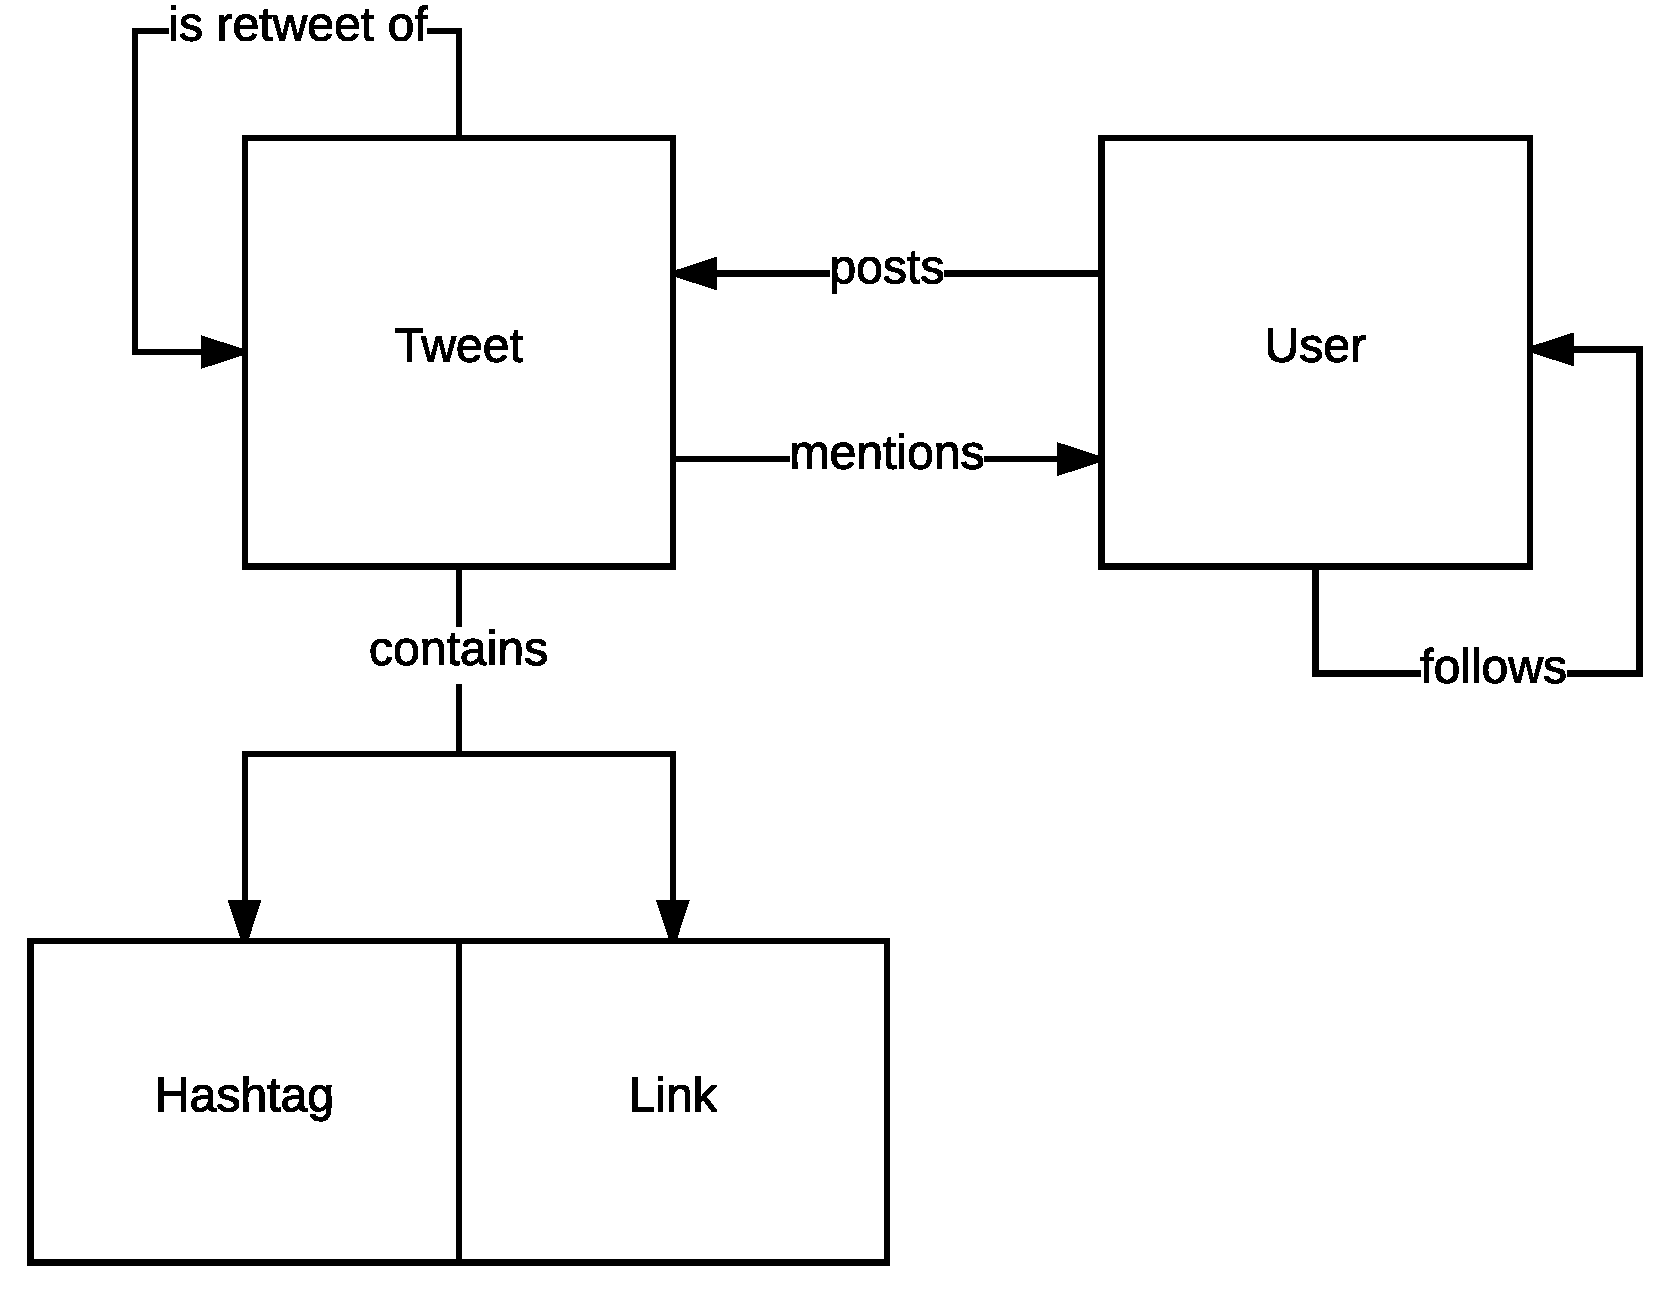
\includegraphics[width=10cm]{../figures/twitter_er.pdf}
\end{figure}

\par
% TODO statuses/tweets persistence
This thesis will focus on analyzing statuses in real time.
Statuses on Twitter can not only contain text, but also rich media like images, gifs, or videos, as well as surveys.
The text itself can also contain links, mention other users by containing \texttt{@<user_name>},
and contain any number of the infamous hashtag (\texttt{#hastag}), used to label a status, all while being limited to 140 characters.
A status can also be a so-called retweet of another status, adding to its content and exposing the other status to the retweeting users' followers.
Research shows that statuses are mostly retweeted shortly after they are published, and often lead to chains of retweets,
which not only spreads information fast, but also diffuses it~\ref{Kwak2010}.\\
As mentioned in~\ref{ch:goals}, one of the goals of this thesis is to be able to observe and detect such a spreading in real time
and analyze its influence on the overall userbase.
\par
For the purpose of this thesis we will only focus on the text of a status and do not assign any special meaning to links,
mentions, hashtags or whether a status is a retweet.\\

% TODO add that retweets mean nothing has to be weighed by likes or something to get sentiment

\section{The Twitter API}
\label{sec:theApi}

Twitter is offering an API (\textbf{A}pplication \textbf{P}rogramming \textbf{I}nterface),
through which developers and researchers can access machine-readable data,
including the entities shown in~\ref{fig:twitter}, from the platform.
This API transmits data encoded in JSON, and follows the REST-paradigm.
A Python-library called Tweepy, which contains utility functions for interaction with the Twitter API, was used where adequate~\cite{tweepyDocs}.

\subsection{JSON}
\label{subsec:json}

JSON (\textbf{J}ava\textbf{S}cript \textbf{O}bject \textbf{N}otation) is data format originally conceptualized by ECMA international
for the programming language Javascript to be light-weight, human-readable yet easy for machines to generate and parse.
Due to this, and the fact that it uses conventions familiar to developers of C-like languages,
it has since become a widespread data-interchange format with libraries for parsing and generation in many languages~\cite{jsonDocs}.
A small example for an object in this format can be seen in~\ref{code:json}.


%{
%    "apple": {
%        "calories": 123,
%        "contains_allergens": false
%        "types": ["Braeburh", "Cortland"]
%        "grows_on": "tree"
%    },
%    "hazelnut": {
%        "calories": 12,
%        "contains_allergens": true
%        "grows_on": "bush"
%    },
%}

\begin{figure}
    \caption{A shortened JSON representation of a fictional Twitter status}
    \label{code:json}
    \begin{minted}{json}
    % @formatter:off
    {
        "created_at" : "Fri Jan 20 20:04:05 +0000 2017",
        "id" : "123",
        "text" : "@other_user Hello!",
        "entities" : {
                "hashtags" : [],
                "symbols" : [],
                "user_mentions" : [{
                    "screen_name" : "other_user",
                    "name" : "Other User"}],
                "urls" : [] },
        "user" : {
            "name" : "User",
            "screen_name" : "user"
        }
    }
        % @formatter:on
    \end{minted}
\end{figure}

\subsection{REST}
\label{subsec:rest}

The Twitter API follows the REST (\textbf{RE}presentational \textbf{S}tate \textbf{T}ransfer) paradigm.
The REST-paradigm defines a set of architectural rules to ensure interoperability of distributed systems,
like clients and servers on the internet.
To achieve that, among other things,
it defines a set methods that specify different kinds of operations that can be performed on data~\cite{Jakl2008}.
The most prevalent methods mentioned in the RFC are listed below~\cite{RFC2616}.

\begin{enumerate}
    \item
    \texttt{GET} - retrieves data identified by the URI (idempotent)
    \item
    \texttt{POST} - request to create a new entity, with the type specified by the URI
    \item
    \texttt{PUT} - request to create an entity identified by the URL, or update it if it exists (idempotent)
    \item
    \texttt{DELETE} - request to delete an entity identified by the URL (idempotent)
\end{enumerate}

There are more methods specified by the RFC~\cite{RFC2616} that will not be used in this thesis.
\par
The resources (also called API endpoints) offered by the Twitter REST-API are rate-limit,
which means any one application or Twitter-user using the API can make a limit number of requests to the API.
Every request send to the API needs to be authenticated,
either as a Twitter user or as an application that can be registered in Twitter's developer console.
Furthermore, there are some resources which can only be accessed when a specific Twitter user authenticates
against the API, because they are user-specific, like publishing a status.
Some examples can be seen in ~\ref{tab:twitter_endpoints}.
% TODO this would be a good place to elaborate some more
% TODO the rate limiting part, for example, is kind of lost int here

\begin{table}
    \caption{A selection of resources offered by the Twitter REST API~\cite{twitterDocs}}
    \label{tab:twitter_endpoints}
    \resizebox{\textwidth}{!}{%
    \begin{tabular}{lllll} %
        \toprule
        & & \multicolumn{2}{c}{Authentication} & \\
        \cmidrule{3-4}
        Method
        & URI
        & User
        & Application
        & Description
        \\
        \midrule
        \texttt{GET}
        & \texttt{search/tweets}
        & \cmark
        & \cmark
        & Returns statuses matching a query
        \\
        \midrule
        \texttt{GET}
        & \texttt{direct_messages}
        & \cmark
        & \xmark
        & Returns direct messages of the authenticated user
        \\
        \midrule
        \texttt{POST}
        & \texttt{statuses/update}
        & \cmark
        & \xmark
        & Posts a status for the authenticated user
        \\
        \bottomrule
    \end{tabular}}
\end{table}

\subsection{Processing Data at Rest and Data in Motion}
\label{subsec:dataAtRest-DataInMotion}

The previous subsection discussed the data at rest offered by the Twitter API.
Processing data at rest (not to be confused with REST) is processing data from a persistent data storage, like a database, in batches~\cite{Nandi2015}.
Since this thesis aims to provide analysis in real time, one option would be to request the latest entities in fixed intervals from
Twitters API.
\par
However, that would be inefficient, and introduces latency to the analysis,
since events like the posting of statuses can only be analyzed after the next request is answered, not immediately when they occur.
This is amplified by the fact that the number of requests than can be made to the API is limited by the rate-limit.
\par
To analyze events right when they occur, the data has to be processed in motion, meaning ingesting data in real time via a stream~\cite{Nandi2015}.
This thesis aims to process data in motion.
Thankfully, Twitter offers a Streaming API, which is explained in the next subsection. % TODO is it okay to reference chapters and stuff like this?


\subsection{Streaming}
\label{subsec:streaming}

Although the Twitter documentation distinguishes between the REST API for processing data at rest and the the Streaming API for processing data in motion,
the streaming API is also REST-based.
The user sends a HTTP-request to a streaming-endpoint, but the the API doesn't respond and close the requests,
but instead keeps the connection open and sends successive responses until the connection closes.
These responses have the same format as in the REST-API, and represent Twitter entities like statuses or direct messages~\cite{twitterDocs}.
A diagram from the Twitter documentation visualizing this behaviour can be seen in~\ref{fig:twitter_streaming}.

% include diagram
\begin{figure}
    \centering
    \caption{Diagram from the Twitter documentation showing how the Twitter streaming-API works}
    \label{fig:twitter_streaming}
    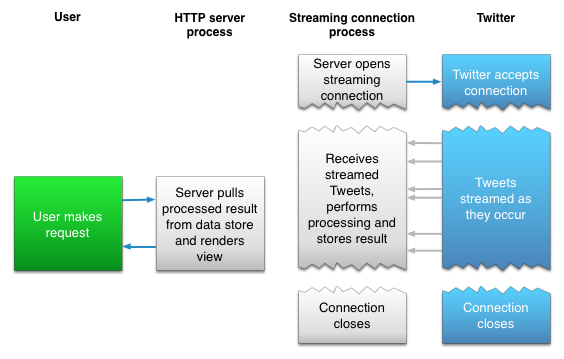
\includegraphics[width=10cm]{../images/twitter_streaming_diagram.png}
\end{figure}


Twitter itself offers 6 different endpoints for 6 different streams, all of which are explained in~\ref{tab:twitter_streams}.

\begin{table}
    \caption{All streams offered by Twitter~\cite{twitterDocs}}
    \label{tab:twitter_streams}
    \resizebox{\textwidth}{!}{%
    \begin{tabular}{lllll} %
        \toprule
        & & \multicolumn{2}{c}{Authentication} & \\
        \cmidrule{3-4}
        Name
        & Method
        & URI
        & User
        & Application
        & Description
        \\
        \midrule
        Filter stream
        & \texttt{POST}
        & \texttt{statuses/filter}
        & \cmark
        & \cmark
        & Streams a random sample of statuses matching the filter setting
        \\
        \midrule
        Sample stream
        & \texttt{GET}
        & \texttt{statuses/sample}
        & \cmark
        & \cmark
        & Streams a random sample of statuses
        \\
        \midrule
        User stream
        & \texttt{GET}
        & \texttt{user}
        & \cmark
        & \xmark
        & Streams all activity regarding the authenticated user
        \\
        \midrule
        Site stream
        & \texttt{GET}
        & \texttt{site}
        & & &
        \\
        \cmidrule{2-3}
        Retweet stream
        & \multicolumn{2}{c}{Unknown}
        & \multicolumn{2}{c}{Not publicly available, disregarded in this thesis} &
        \\
        \cmidrule{2-3}
        Firehose
        & \multicolumn{2}{c}{Unknown}
        & & &
        \\
        \bottomrule
    \end{tabular}}
\end{table}

This thesis will work with the sample, user and filter stream, since only these are publicly available.
The main focus will be the sample stream, since it gives a representative sample of all activity on twitter.
\par
Compared to the general use-case for Kafka shown in~\ref{fig:kafka}, in this thesis,
every producer will produce events for exactly one topic, with the producer being a specific Twitter stream and the topic beint a unique identifier for it.
%TODO maybe show adjusted diagram here if its not clear
The advantage of using the Twitter streaming-API compared to repeatedly polling the REST-API for the use-case of this thesis
is that it is more efficient and has less latency.

\section{The Sanders Dataset}
\label{sec:theSandersDataset}

To train the sentiment analysis models, a set of statuses labeled with sentiment was needed.
Evaluation using the comparison in\cite{Saif2013} showed the Sanders-dataset \cite{sanders} to be most-suited to train twitter sentiment analysis models.
It is large enough to train an accurate model and is hand-labeled instead of relying on emoticons for labeling, which might be inaccurate.
Also, Twitter's terms of service forbid the distribution of statuses outside of their API, which ruled out all datasets that did.
The Sanders-dataset only contains the statuses unique identifier (id), along with the sentiment label ("positive", "negative", "neutral" or "irrelevant").
The existing scripts to hydrate the dataset (replace the id with the actual status by requesting them from the API) were either slow or deprecated and dysfunctional,
which is why a new script was written.
Unfortunately no real statuses can be shown, but~\ref{tab:sanders_sample} shows some fictional examples.

\begin{table}
    \caption{Some fictional statuses with labels}
    \label{tab:sanders_sample}
    \resizebox{\textwidth}{!}{%
    \begin{tabular}{lllll} %
        \toprule
        Text
        & Sentiment Label
        \\
        \midrule
        Lmao I had a funny argument with Siri @Apple
        & \texttt{positive}
        \\
        My #iPad crashes constantly since the update.
        & \texttt{negative}
        \\
        Can anyone recommend me an app for my iPhone?
        & \texttt{neutral}
        \\
        Apple stellt neues iPhone vor \textit{(non-english)}
        & \texttt{irrelevant}
        \bottomrule
    \end{tabular}}
\end{table}

The resulting dataset was then filtered to only contain english statuses.
The distribution of labels on the dataset can be seen in~\ref{fig:sanders_sentiment}.

% include diagram
\begin{figure}
    \centering
    \caption{The distribution of labels in the Sanders dataset.}
    \label{fig:sanders_sentiment}
    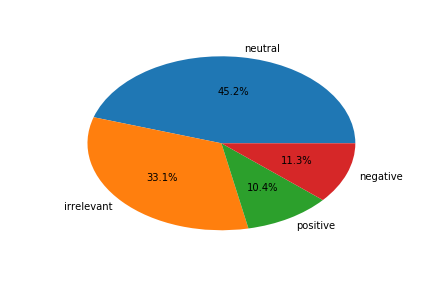
\includegraphics[width=10cm]{../images/sanders_sentiment.png}
\end{figure}

\section{The Streaming Sample Dataset}
\label{sec:streamingSampleDataset}

Another dataset was collected by streaming the sample stream described in\ref{subsec:streaming},
again only keeping english tweets.
The statuses received via the stream were written to a database until 10000 statuses were collected.
This dataset will be used for (unsupervised) topic modeling, since it is representative of all activity on Twitter.
A wordcloud of the statuses collected from the sample stream can be seen in~\ref{fig:wordloud_pre}~

% include diagram
\begin{figure}
    \centering
    \caption{Wordcloud of the statuses collected from the sample stream.}
    \label{fig:wordloud_pre}
    \includegraphics[width=10cm]{../images/wordloud_pre.png}
\end{figure}

Some of the biggest "words" in the wordcloud are "RT", "it" and "be",
or even some digits, which have no informativeness with regards to sentiment or topic,
which demonstrates the necessity of preprocessing, shown in the next chapter.


\section{Preprocessing and Tokenization}
\label{sec:preprocessingAndTokenization}

There are now 2 datasets of statuses that are filtered by language but still raw.
These statuses now need to be preprocessed,
which in this case means removing all elements of text that have no influence on topic and sentiment and make
modeling and analysis unnecessarily difficult.\\
Furthermore, since all the algorithms that will be used later on are bag-of-words algorithms,
which means they disregard the order of words in text, a tokenization function needs to be created
to split sentences in the right places and only keep tokens (words) relevant for modeling and analysis.\\
However, to achieve consistent results,
the same preprocessing and tokenization functions need to be used for all models, analyses and datasets.
The following steps were taken.

\begin{enumerate}
    \item Precrocessing
    \begin{enumerate}
        \item All URL's were removed by using a regular expression matching everything from "http" up to the next whitespace
        \item All punctuation as well as the Twitter-specific characters \texttt{@} and \texttt{#} were removed
        \item The text was split at whitespace using the \texttt{\\s} regular expression
        \item All elements that contained anything but latin letters were discarded
    \end{enumerate}
    \item Tokenization
    \begin{enumerate}
        \item The text is split into tokens using the whitespace regular expression again
        \item Tokens of length 1 are removed
        \item Tokens that can be found in NLTK's stopwords list for the english language
        (containing a fixed selection of words with low-informativeness for bag-of-words algorithms) were removed
        \item Tokens that can be found in an additional self-devised stopwords list were removed % TODO put this stopword list plus the code in the appendix and reference it here
    \end{enumerate}
\end{enumerate}

The change to the wordcloud of the statuses collected from the sample stream after preprocessing and tokenization can be seen in~\ref{fig:wordloud_post}.

\begin{figure}
    \centering
    \caption{Wordcloud of the statuses collected from the sample stream after preprocessing and tokenization.}
    \label{fig:wordloud_post}
    \includegraphics[width=10cm]{../images/wordloud_post.png}
\end{figure}

%TODO be more specific what is used where here
The preprocessed datasets were saved to be used later.
Also, two dictionaries of the preprocessed datasets were made using the Gensim-library,
which will be explained in more detail in\ref{ch:topicModeling}~ where the library is primarily used.
The dictionaries will be used for sentiment analysis and topic modeling.
